\documentclass[border=4pt]{standalone}
\usepackage{tikz}
\usepackage{amsmath,amssymb}
\usetikzlibrary{arrows.meta,shapes.geometric}

\definecolor{steelblue}{RGB}{51,115,199}
\definecolor{amber}{RGB}{217,140,26}
\definecolor{teal}{RGB}{26,166,89}
\definecolor{coral}{RGB}{217,38,38}
\definecolor{panelbg}{RGB}{244,244,244}
\definecolor{subpanelbg}{RGB}{237,237,237}
\definecolor{darktext}{RGB}{30,30,30}
\definecolor{midgray}{RGB}{130,130,130}
\definecolor{arrowblue}{RGB}{80,140,215}

\begin{document}
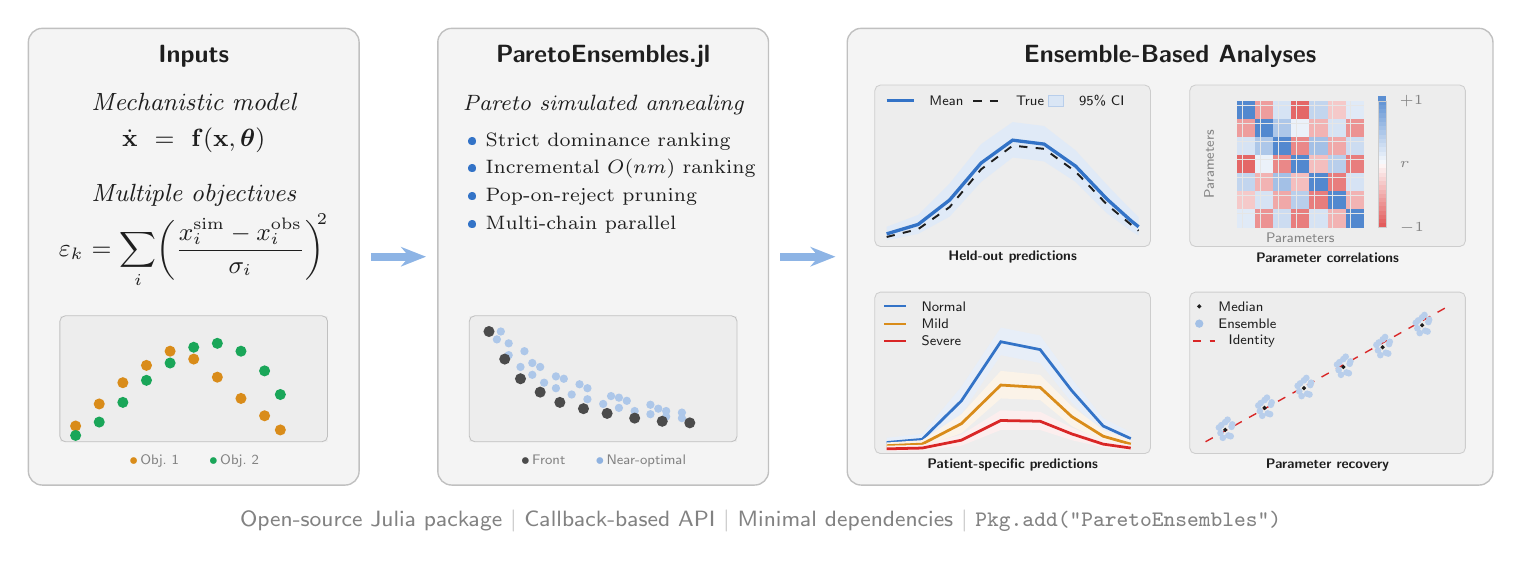
\begin{tikzpicture}[>=Stealth, every node/.style={font=\sffamily}]

\def\ph{5.8}
\def\pw{4.2}
\def\rpw{8.2}
\def\pAx{0}
\def\pBx{5.2}
\def\pCx{10.4}

% ════════════════════════════════════════════
% Panel backgrounds
% ════════════════════════════════════════════
\fill[panelbg, rounded corners=5pt, draw=midgray!50, line width=0.5pt]
    (\pAx, 0) rectangle +(\pw, \ph);
\fill[panelbg, rounded corners=5pt, draw=midgray!50, line width=0.5pt]
    (\pBx, 0) rectangle +(\pw, \ph);
\fill[panelbg, rounded corners=5pt, draw=midgray!50, line width=0.5pt]
    (\pCx, 0) rectangle +(\rpw, \ph);

% ════════════════════════════════════════════
% PANEL 1: INPUTS
% ════════════════════════════════════════════
\node[font=\sffamily\bfseries\small, text=darktext]
    at (\pAx + \pw/2, \ph - 0.35) {Inputs};

\node[anchor=north, text width=3.6cm, align=center, font=\small, text=darktext]
    at (\pAx + \pw/2, \ph - 0.7) {%
    {\itshape Mechanistic model}\\[2pt]
    $\dot{\mathbf{x}} = \mathbf{f}(\mathbf{x}, \boldsymbol{\theta})$%
};

\node[anchor=north, text width=3.6cm, align=center, font=\small, text=darktext]
    at (\pAx + \pw/2, \ph - 1.85) {%
    {\itshape Multiple objectives}\\[2pt]
    $\displaystyle\varepsilon_k = \sum_i \!\left(\frac{x_i^{\text{sim}} - x_i^{\text{obs}}}{\sigma_i}\right)^{\!\!2}$%
};

% Training data mini-plot
\begin{scope}[shift={(\pAx + 0.4, 0.55)}, clip]
    \clip (0,0) rectangle (3.4, 1.6);
    \fill[subpanelbg] (0,0) rectangle (3.4, 1.6);
    \foreach \x/\y in {0.2/0.2, 0.5/0.48, 0.8/0.75, 1.1/0.97, 1.4/1.15, 1.7/1.05, 2.0/0.82, 2.3/0.55, 2.6/0.33, 2.8/0.15} {
        \fill[amber] (\x,\y) circle (2pt);
    }
    \foreach \x/\y in {0.2/0.08, 0.5/0.25, 0.8/0.5, 1.1/0.78, 1.4/1.0, 1.7/1.2, 2.0/1.25, 2.3/1.15, 2.6/0.9, 2.8/0.6} {
        \fill[teal] (\x,\y) circle (2pt);
    }
\end{scope}
\draw[midgray!50, line width=0.3pt, rounded corners=2pt]
    (\pAx + 0.4, 0.55) rectangle ++(3.4, 1.6);
\node[font=\sffamily\tiny, text=midgray] at (\pAx + \pw/2, 0.3) {%
    \textcolor{amber}{$\bullet$}\;\!Obj.\ 1\qquad
    \textcolor{teal}{$\bullet$}\;\!Obj.\ 2%
};

% ════════════════════════════════════════════
% PANEL 2: ALGORITHM
% ════════════════════════════════════════════
\node[font=\sffamily\bfseries\small, text=darktext]
    at (\pBx + \pw/2, \ph - 0.35) {ParetoEnsembles.jl};

\node[anchor=north, align=center, font=\footnotesize\itshape, text=darktext]
    at (\pBx + \pw/2, \ph - 0.72) {Pareto simulated annealing};

\node[anchor=north west, text width=3.8cm, align=left, font=\scriptsize, text=darktext]
    at (\pBx + 0.25, \ph - 1.2) {%
    \raggedright
    \textcolor{steelblue}{\textbullet}~Strict dominance ranking\\[2pt]
    \textcolor{steelblue}{\textbullet}~Incremental $O(nm)$ ranking\\[2pt]
    \textcolor{steelblue}{\textbullet}~Pop-on-reject pruning\\[2pt]
    \textcolor{steelblue}{\textbullet}~Multi-chain parallel%
};

% Mini Pareto front
\begin{scope}[shift={(\pBx + 0.4, 0.55)}, clip]
    \clip (0,0) rectangle (3.4, 1.6);
    \fill[subpanelbg] (0,0) rectangle (3.4, 1.6);
    \foreach \x/\y in {
        0.35/1.3, 0.5/1.1, 0.65/0.95, 0.8/0.85, 0.95/0.75,
        1.1/0.68, 1.3/0.6, 1.5/0.54, 1.7/0.48, 1.9/0.43,
        2.1/0.39, 2.3/0.35, 2.5/0.32, 2.7/0.3,
        0.5/1.25, 0.8/1.0, 1.1/0.83, 1.5/0.68, 1.9/0.56,
        2.3/0.47, 2.7/0.37, 0.4/1.4, 0.9/0.95, 1.4/0.73,
        2.0/0.52, 2.5/0.39, 0.7/1.15, 1.2/0.8, 1.8/0.58, 2.4/0.42
    } {
        \fill[steelblue!40] (\x, \y) circle (1.5pt);
    }
    \foreach \x/\y in {
        0.25/1.4, 0.45/1.05, 0.65/0.8, 0.9/0.63, 1.15/0.5,
        1.45/0.42, 1.75/0.36, 2.1/0.3, 2.45/0.26, 2.8/0.24
    } {
        \fill[darktext!80] (\x, \y) circle (2pt);
    }
\end{scope}
\draw[midgray!50, line width=0.3pt, rounded corners=2pt]
    (\pBx + 0.4, 0.55) rectangle ++(3.4, 1.6);
\node[font=\sffamily\tiny, text=midgray] at (\pBx + \pw/2, 0.3) {%
    \textcolor{darktext!80}{$\bullet$}\;\!Front\qquad
    \textcolor{steelblue!55}{$\bullet$}\;\!Near-optimal%
};

% ════════════════════════════════════════════
% PANEL 3: OUTPUTS — 2×2 grid
% ════════════════════════════════════════════
\node[font=\sffamily\bfseries\small, text=darktext]
    at (\pCx + \rpw/2, \ph - 0.35) {Ensemble-Based Analyses};

\def\spw{3.5}
\def\sph{2.05}
\def\spcol{0.5}
\def\splm{0.35}

\pgfmathsetmacro{\spLx}{\pCx + \splm}
\pgfmathsetmacro{\spRx}{\pCx + \splm + \spw + \spcol}
\pgfmathsetmacro{\topRowY}{\ph - 0.72 - \sph}
\pgfmathsetmacro{\botRowY}{\topRowY - 0.58 - \sph}

% ────────────────────────────────────────────
% Top-left: Held-out predictions
% ────────────────────────────────────────────
\fill[subpanelbg, rounded corners=2pt] (\spLx, \topRowY) rectangle ++(\spw, \sph);
\draw[midgray!40, line width=0.3pt, rounded corners=2pt] (\spLx, \topRowY) rectangle ++(\spw, \sph);
\begin{scope}[shift={(\spLx, \topRowY)}, clip]
    \clip (0,0) rectangle (\spw, \sph);
    \fill[steelblue!15]
        (0.15,0.25) -- (0.55,0.4) -- (0.95,0.8) -- (1.35,1.3) -- (1.75,1.58) -- (2.15,1.53) -- (2.55,1.22) -- (2.95,0.78) -- (3.25,0.47) -- (3.35,0.37)
        -- (3.35,0.14) -- (3.25,0.2) -- (2.95,0.42) -- (2.55,0.82) -- (2.15,1.08) -- (1.75,1.13) -- (1.35,0.82) -- (0.95,0.38) -- (0.55,0.16) -- (0.15,0.08) -- cycle;
    \draw[steelblue, line width=1.2pt]
        (0.15,0.16) -- (0.55,0.28) -- (0.95,0.59) -- (1.35,1.06) -- (1.75,1.35) -- (2.15,1.3) -- (2.55,1.02) -- (2.95,0.6) -- (3.25,0.33) -- (3.35,0.25);
    \draw[darktext, line width=0.7pt, dashed]
        (0.15,0.12) -- (0.55,0.22) -- (0.95,0.5) -- (1.35,0.98) -- (1.75,1.28) -- (2.15,1.24) -- (2.55,0.95) -- (2.95,0.53) -- (3.25,0.28) -- (3.35,0.2);
\end{scope}
% Legend inside sub-panel, top-left (low-data region)
\pgfmathsetmacro{\predLegY}{\topRowY + \sph - 0.2}
\pgfmathsetmacro{\predLegX}{\spLx + 0.15}
\draw[steelblue, line width=1pt] (\predLegX, \predLegY) -- ++(0.35, 0);
\node[font=\sffamily\tiny, text=darktext, anchor=west] at ({\predLegX + 0.42}, \predLegY) {Mean};
\draw[darktext, line width=0.6pt, dashed] ({\predLegX + 1.1}, \predLegY) -- ++(0.35, 0);
\node[font=\sffamily\tiny, text=darktext, anchor=west] at ({\predLegX + 1.52}, \predLegY) {True};
\fill[steelblue!18] ({\predLegX + 2.05}, {\predLegY - 0.07}) rectangle ++(0.2, 0.14);
\draw[steelblue!35, line width=0.25pt] ({\predLegX + 2.05}, {\predLegY - 0.07}) rectangle ++(0.2, 0.14);
\node[font=\sffamily\tiny, text=darktext, anchor=west] at ({\predLegX + 2.32}, \predLegY) {95\% CI};
% Title
\node[font=\sffamily\tiny\bfseries, text=darktext] at ({\spLx + \spw/2}, {\topRowY - 0.14}) {Held-out predictions};

% ────────────────────────────────────────────
% Top-right: Parameter correlations
% ────────────────────────────────────────────
\fill[subpanelbg, rounded corners=2pt] (\spRx, \topRowY) rectangle ++(\spw, \sph);
\draw[midgray!40, line width=0.3pt, rounded corners=2pt] (\spRx, \topRowY) rectangle ++(\spw, \sph);
% Heatmap grid - compute positions OUTSIDE clip for labels
\def\cs{0.23}
\pgfmathsetmacro{\hmox}{\spRx + 0.6}
\pgfmathsetmacro{\hmoy}{\topRowY + (\sph - 7*\cs)/2 + 0.02}
\pgfmathsetmacro{\hmRight}{7*\cs + \hmox}
\pgfmathsetmacro{\hmTop}{7*\cs + \hmoy}
% Draw heatmap (clipped to sub-panel)
\begin{scope}[clip]
    \clip (\spRx, \topRowY) rectangle ++(\spw, \sph);
    \foreach \i/\j/\c in {
        0/6/steelblue!85, 1/6/coral!45,    2/6/steelblue!20, 3/6/coral!70,    4/6/steelblue!30, 5/6/coral!25, 6/6/steelblue!15,
        0/5/coral!45,     1/5/steelblue!85, 2/5/steelblue!40, 3/5/steelblue!10,4/5/coral!35,     5/5/steelblue!20, 6/5/coral!50,
        0/4/steelblue!20, 1/4/steelblue!40, 2/4/steelblue!85, 3/4/coral!55,    4/4/steelblue!45, 5/4/coral!40, 6/4/steelblue!25,
        0/3/coral!70,     1/3/steelblue!10, 2/3/coral!55,     3/3/steelblue!85,4/3/coral!30,     5/3/steelblue!35, 6/3/coral!60,
        0/2/steelblue!30, 1/2/coral!35,     2/2/steelblue!45, 3/2/coral!30,    4/2/steelblue!85, 5/2/coral!60, 6/2/steelblue!20,
        0/1/coral!25,     1/1/steelblue!20, 2/1/coral!40,     3/1/steelblue!35,4/1/coral!60,     5/1/steelblue!85, 6/1/coral!35,
        0/0/steelblue!15, 1/0/coral!50,     2/0/steelblue!25, 3/0/coral!60,    4/0/steelblue!20, 5/0/coral!35, 6/0/steelblue!85
    } {
        \fill[\c] ({\i*\cs+\hmox}, {\j*\cs+\hmoy}) rectangle +({\cs}, {\cs});
    }
    \draw[midgray!20, line width=0.15pt, step=\cs]
        (\hmox, \hmoy) grid (\hmRight, \hmTop);
\end{scope}
% Axis labels (outside clip, won't be cut)
\node[font=\sffamily\tiny, text=midgray, rotate=90, anchor=south]
    at ({\hmox - 0.17}, {\hmoy + 3.5*\cs}) {Parameters};
\node[font=\sffamily\tiny, text=midgray]
    at ({\hmox + 3.5*\cs}, {\hmoy - 0.13}) {Parameters};
% Color bar (outside clip)
\pgfmathsetmacro{\cbx}{\hmRight + 0.18}
\pgfmathsetmacro{\cbbot}{\hmoy}
\pgfmathsetmacro{\cbh}{7*\cs}
\foreach \k in {0,...,30} {
    \pgfmathsetmacro{\yy}{\cbbot + \k*\cbh/30}
    \ifnum\k<15
        \fill[coral!\the\numexpr 75 - \k*5\relax] (\cbx, \yy) rectangle ++(0.1, {\cbh/30 + 0.003});
    \else
        \fill[steelblue!\the\numexpr (\k-15)*5 + 5\relax] (\cbx, \yy) rectangle ++(0.1, {\cbh/30 + 0.003});
    \fi
}
\draw[midgray!40, line width=0.2pt] (\cbx, \cbbot) rectangle ++(0.1, \cbh);
\node[font=\sffamily\tiny, text=midgray, anchor=west] at ({\cbx + 0.15}, \cbbot) {$-1$};
\node[font=\sffamily\tiny, text=midgray, anchor=west] at ({\cbx + 0.15}, {\cbbot + \cbh/2}) {$r$};
\node[font=\sffamily\tiny, text=midgray, anchor=west] at ({\cbx + 0.15}, {\cbbot + \cbh}) {$+1$};
% Title
\node[font=\sffamily\tiny\bfseries, text=darktext] at ({\spRx + \spw/2}, {\topRowY - 0.14}) {Parameter correlations};

% ────────────────────────────────────────────
% Bottom-left: Patient-specific predictions
% ────────────────────────────────────────────
\fill[subpanelbg, rounded corners=2pt] (\spLx, \botRowY) rectangle ++(\spw, \sph);
\draw[midgray!40, line width=0.3pt, rounded corners=2pt] (\spLx, \botRowY) rectangle ++(\spw, \sph);
\begin{scope}[shift={(\spLx, \botRowY)}, clip]
    \clip (0,0) rectangle (\spw, \sph);
    % Normal (blue)
    \fill[steelblue!12]
        (0.15,0.2) -- (0.6,0.25) -- (1.1,0.85) -- (1.6,1.6) -- (2.1,1.5) -- (2.5,0.95) -- (2.9,0.45) -- (3.25,0.27)
        -- (3.25,0.12) -- (2.9,0.25) -- (2.5,0.65) -- (2.1,1.15) -- (1.6,1.25) -- (1.1,0.5) -- (0.6,0.12) -- (0.15,0.08) -- cycle;
    \draw[steelblue, line width=1pt]
        (0.15,0.14) -- (0.6,0.18) -- (1.1,0.67) -- (1.6,1.42) -- (2.1,1.32) -- (2.5,0.8) -- (2.9,0.35) -- (3.25,0.19);
    % Mild (amber)
    \fill[amber!10]
        (0.15,0.14) -- (0.6,0.17) -- (1.1,0.5) -- (1.6,1.05) -- (2.1,1.0) -- (2.5,0.6) -- (2.9,0.3) -- (3.25,0.17)
        -- (3.25,0.08) -- (2.9,0.15) -- (2.5,0.35) -- (2.1,0.68) -- (1.6,0.7) -- (1.1,0.26) -- (0.6,0.08) -- (0.15,0.06) -- cycle;
    \draw[amber, line width=1pt]
        (0.15,0.1) -- (0.6,0.12) -- (1.1,0.38) -- (1.6,0.87) -- (2.1,0.84) -- (2.5,0.47) -- (2.9,0.22) -- (3.25,0.12);
    % Severe (coral)
    \fill[coral!8]
        (0.15,0.1) -- (0.6,0.11) -- (1.1,0.24) -- (1.6,0.55) -- (2.1,0.53) -- (2.5,0.33) -- (2.9,0.17) -- (3.25,0.11)
        -- (3.25,0.04) -- (2.9,0.08) -- (2.5,0.17) -- (2.1,0.3) -- (1.6,0.3) -- (1.1,0.1) -- (0.6,0.04) -- (0.15,0.03) -- cycle;
    \draw[coral, line width=1pt]
        (0.15,0.06) -- (0.6,0.07) -- (1.1,0.17) -- (1.6,0.42) -- (2.1,0.41) -- (2.5,0.25) -- (2.9,0.12) -- (3.25,0.07);
\end{scope}
% Legend inside, top-left corner (before curves rise)
\pgfmathsetmacro{\psLX}{\spLx + 0.12}
\pgfmathsetmacro{\psLY}{\botRowY + \sph - 0.18}
\draw[steelblue, line width=0.8pt] (\psLX, \psLY) -- ++(0.28, 0);
\node[font=\sffamily\tiny, text=darktext, anchor=west] at ({\psLX + 0.35}, \psLY) {Normal};
\draw[steelblue, line width=0.8pt] (\psLX, {\psLY - 0.22}) -- ++(0.28, 0);
\draw[amber, line width=0.8pt] (\psLX, {\psLY - 0.22}) -- ++(0.28, 0);
\node[font=\sffamily\tiny, text=darktext, anchor=west] at ({\psLX + 0.35}, {\psLY - 0.22}) {Mild};
\draw[coral, line width=0.8pt] (\psLX, {\psLY - 0.44}) -- ++(0.28, 0);
\node[font=\sffamily\tiny, text=darktext, anchor=west] at ({\psLX + 0.35}, {\psLY - 0.44}) {Severe};
% Title
\node[font=\sffamily\tiny\bfseries, text=darktext] at ({\spLx + \spw/2}, {\botRowY - 0.14}) {Patient-specific predictions};

% ────────────────────────────────────────────
% Bottom-right: Parameter recovery
% ────────────────────────────────────────────
\fill[subpanelbg, rounded corners=2pt] (\spRx, \botRowY) rectangle ++(\spw, \sph);
\draw[midgray!40, line width=0.3pt, rounded corners=2pt] (\spRx, \botRowY) rectangle ++(\spw, \sph);
\begin{scope}[shift={(\spRx, \botRowY)}, clip]
    \clip (0,0) rectangle (\spw, \sph);
    \draw[coral, line width=0.5pt, dashed] (0.2,0.15) -- (3.3,1.88);
    \foreach \cx/\cy in {0.45/0.3, 0.95/0.58, 1.45/0.83, 1.95/1.1, 2.45/1.35, 2.95/1.63} {
        \foreach \dx/\dy in {0/0.1, 0.07/-0.08, -0.05/0.06, 0.08/0.04, -0.06/-0.04, 0.03/0.13, -0.03/-0.1, 0.09/0.07, -0.08/0.03, 0.04/-0.07} {
            \fill[steelblue!35] ({\cx+\dx}, {\cy+\dy}) circle (1.2pt);
        }
        \node[diamond, fill=darktext, inner sep=0.4pt, minimum size=1.8pt] at (\cx, \cy) {};
    }
\end{scope}
% Legend inside, top-left corner (stacked vertically like patient panel)
\pgfmathsetmacro{\prLX}{\spRx + 0.12}
\pgfmathsetmacro{\prLY}{\botRowY + \sph - 0.18}
\node[diamond, fill=darktext, inner sep=0.35pt, minimum size=1.8pt] at (\prLX, \prLY) {};
\node[font=\sffamily\tiny, text=darktext, anchor=west] at ({\prLX + 0.12}, \prLY) {Median};
\fill[steelblue!45] (\prLX, {\prLY - 0.22}) circle (1.5pt);
\node[font=\sffamily\tiny, text=darktext, anchor=west] at ({\prLX + 0.12}, {\prLY - 0.22}) {Ensemble};
\draw[coral, line width=0.5pt, dashed] ({\prLX - 0.08}, {\prLY - 0.44}) -- ++(0.28, 0);
\node[font=\sffamily\tiny, text=darktext, anchor=west] at ({\prLX + 0.25}, {\prLY - 0.44}) {Identity};
% Title
\node[font=\sffamily\tiny\bfseries, text=darktext] at ({\spRx + \spw/2}, {\botRowY - 0.14}) {Parameter recovery};

% ════════════════════════════════════════════
% ARROWS
% ════════════════════════════════════════════
\pgfmathsetmacro{\arrowY}{\ph/2}
\draw[-{Stealth[length=9pt,width=7pt]}, line width=3pt, color=arrowblue!65]
    (\pAx + \pw + 0.15, \arrowY) -- (\pBx - 0.15, \arrowY);
\draw[-{Stealth[length=9pt,width=7pt]}, line width=3pt, color=arrowblue!65]
    (\pBx + \pw + 0.15, \arrowY) -- (\pCx - 0.15, \arrowY);

% ════════════════════════════════════════════
% Bottom tagline
% ════════════════════════════════════════════
\pgfmathsetmacro{\figcenter}{(\pCx + \rpw)/2}
\node[font=\sffamily\footnotesize, text=midgray] at (\figcenter, -0.45) {
    Open-source Julia package \textcolor{midgray!50}{$\vert$}\
    Callback-based API \textcolor{midgray!50}{$\vert$}\
    Minimal dependencies \textcolor{midgray!50}{$\vert$}\
    \texttt{Pkg.add("ParetoEnsembles")}
};

\end{tikzpicture}
\end{document}
